\section{Introduction}
\subsection{LIGO and Gravitational Wave Detection}
\begin{figure}[htbp]
\begin{center}
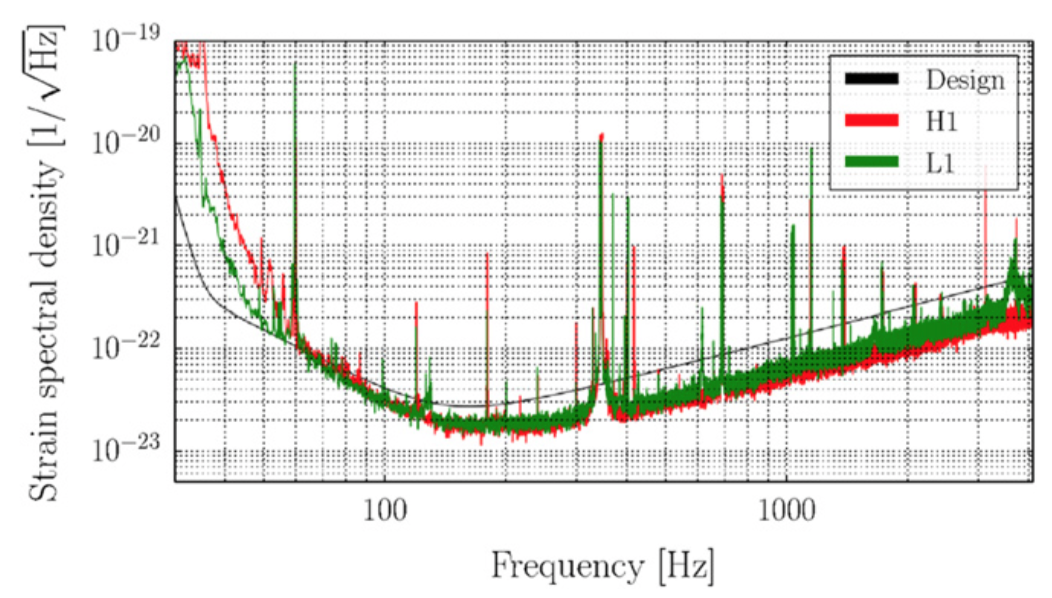
\includegraphics[width=\textwidth]{sencurve}
\caption{Sensitivity curve for LIGO S6 run as a function of frequency.}
\label{sencurve}
\end{center}
\end{figure}

GWs, distortions in space emitted from asymmetric accelerations, are one of the implications of Einstein's general relativity. A century after general relativity, searches for direct detection of GWs are still active and are currently being led by the Laser Interferometer Gravitational-wave Observatory (LIGO) Scientific Collaboration (LSC) and VIRGO Collaboration. 

\par{}
LIGO operates two detectors in Louisiana and Washington~\cite{ligo}. The gravitational-wave detector is a simple Michelson interferometer, with Fabry-P\'{e}rot cavities as its 4km interferometric arms. The laser gets reflected repeatedly making an effective length of approximately 300 km per arm. At rest, the laser from the detectors cancels out due to their phase-difference. When a GW passes through the detector, it stretches space in on direction while compressing it another perpendicular direction, resulting in a phase-difference in the interferometer that does not allow the laser reflected from the two mirrors to cancel out~\cite{kip}, and, therefore resulting in the detection of the GW. Using two separate detectors, one can point the detectors to a particular point by setting an appropriate time-delay between the two detectors~\cite{sgwb}, knowing that they travel at the speed of light. In this project, the coordinates of the Sun are used and updated over the period of the analysis to set this time-delay.
\par{}
The sixth LIGO science run data was used in this analysis, which has a maximum strain sensitivity between $10^{-22}$ and $10^{-23}$~\cite{LIGO:2012aa}. Figure~\ref{sencurve} shows the sensitivity curve (amplitude spectral density) as a function of frequency~\cite{newplot}. 

\subsection{Solar MHD Dynamo}
\begin{figure}
\begin{minipage}[c][23cm]{0.9\textwidth}
  \caption{Effect of bandpass-filtering between 100 and 300 Hz}
  \centering
  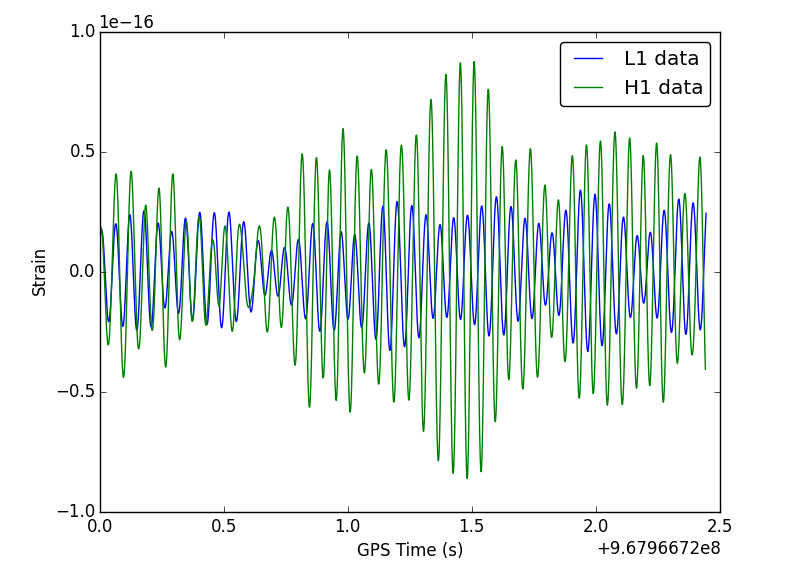
\includegraphics[width=0.95\textwidth]{L1_H1}
  \subcaption{Strain data before filtering}
  \label{figa}
   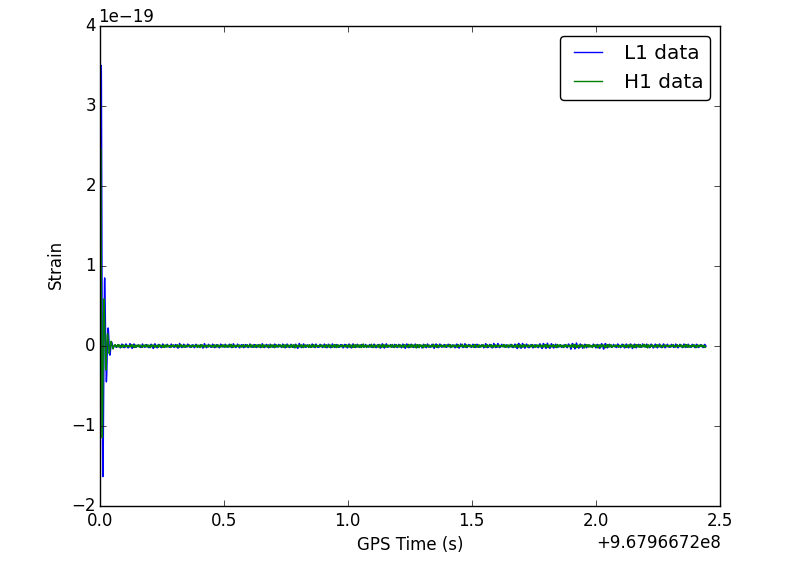
\includegraphics[width=\textwidth]{bandpass}
  \subcaption{Strain data after filtering}
  \label{figb}
\end{minipage}
\end{figure}

Most of the gravitational-wave searches so far target sources such as compact binary systems~\cite{bh1},~\cite{bh2} (black hole, neutron star, or white dwarf binaries), supernovae~\cite{supernovae}, pulsars (continuous waves)~\cite{pulsars}, and the stochastic GW background - the remnant of the big bang~\cite{sgwb},~\cite{sgwb2}. None of these S6 searches reported gravitational-wave detection. Most of the existing theoretical studies~\cite{theory2} as well as simulations~\cite{sim2},~\cite{sim}  also target such sources. In this project, we use the S6 data to study one of the less-traditional sources: the Sun.
\par{}
Winterberg recently conjectured~\cite{winterberg} that the magnetohydrodynamic (MHD) dynamo at the core of the Sun should emit GWs, albeit at a lower frequency than LIGO is most sensitive to. These GWs could theoretically show a strain signal of up to $h = ~10^{-10}$~\cite{winterberg}. Furthermore, these GWs might, themselves, be a noisy background when looking for GWs from more traditional sources that might be preventing their detection. This provides theoretical motivation for our search. 
